% pipeline_v2 (fig:pipeline, figure*): one keyframe update of the UAGS field, with real
% thumbnails. Replaces the formula-only pipeline.tex (kept untouched); design notes in
% docs/reports/2026-10-20-figures-video/logs/pipeline_summary.md.
% Notation follows Sec. III of main.tex; the index n of a Gaussian is dropped except in
% w_{p,n}, f_n and mu_n. Thumbnails (validation scenes only) and values.tex are generated by
% scripts/render_pipeline_thumbs.py: Replica office_0 mapping keyframe 825 (1, 2, 6, 9);
% NeRF-Object-Removal 002, update view 335 (7) and its mapping-pass null (threshold glyph).
% Build (from papers/): pdflatex -output-directory <dir> figs/pipeline_v2.tex
% Natural width = 7.16 in (IEEEtran journal \textwidth): text prints at 7 pt, labels at 6 pt.
\documentclass[tikz,border=0pt]{standalone}
\usepackage[T1]{fontenc}
\renewcommand{\rmdefault}{ptm}          % Times text, CM math: as the paper (IEEEtran)
\usepackage{amsmath,amssymb}
\usepackage{graphicx}
\graphicspath{{figs/pipeline_thumbs/}{pipeline_thumbs/}}
\usetikzlibrary{arrows.meta,calc}

\newcommand{\R}{\mathbf{R}}
\newcommand{\zv}{\mathbf{z}}
\newcommand{\uv}{\mathbf{u}}
\newcommand{\fv}{\mathbf{f}}
\newcommand{\Fv}{\mathbf{F}}
\newcommand{\Yv}{\mathbf{Y}}
\newcommand{\tv}{\mathbf{t}}
\newcommand{\muv}{\boldsymbol{\mu}}
\newcommand{\Sph}{\mathbb{S}}
\newcommand{\old}{\mathrm{old}}
\newcommand{\new}{\mathrm{new}}
\newcommand{\epi}{\mathrm{epi}}
\newcommand{\ale}{\mathrm{ale}}
\newcommand{\sixpt}{\fontsize{6}{7}\selectfont}

% Okabe-Ito
\definecolor{okblue}{HTML}{0072B2}
\definecolor{okorange}{HTML}{E69F00}
\definecolor{okgreen}{HTML}{009E73}
\colorlet{evid}{okblue}
\colorlet{evidtxt}{okblue!85!black}
\colorlet{chg}{okorange!80!black}
\colorlet{chgtxt}{okorange!50!black}
\colorlet{rd}{okgreen!80!black}
\colorlet{rdtxt}{okgreen!55!black}
\definecolor{undefgrey}{gray}{0.72}     % = render_qual.py UNDEF

% generated legend colours / names (scripts/render_pipeline_thumbs.py compose)
\InputIfFileExists{figs/pipeline_thumbs/values.tex}{}{% generated by scripts/render_pipeline_thumbs.py compose; do not edit
\definecolor{labA}{rgb}{0.1216,0.4667,0.7059}
\newcommand{\labnameA}{wall}
\definecolor{labB}{rgb}{1.0000,0.4980,0.0549}
\newcommand{\labnameB}{ceiling}
\definecolor{labC}{rgb}{0.5490,0.3373,0.2941}
\newcommand{\labnameC}{tv-screen}
\definecolor{labD}{rgb}{0.8392,0.1529,0.1569}
\newcommand{\labnameD}{rug}
\newcommand{\nullthetafrac}{0.6250}
}

% step number: white digit on a black disc
\newcommand{\step}[1]{\tikz[baseline=(s.base)]\node[circle,fill=black,text=white,inner sep=0pt,
  minimum size=3.0mm,font=\scriptsize\bfseries](s){#1};}

\begin{document}
\begin{tikzpicture}[
  x=1cm, y=1cm, font=\scriptsize, line cap=round,
  box/.style={draw, rounded corners=2pt, line width=0.55pt, anchor=north west},
  evidbox/.style={box, draw=evid, fill=evid!5},
  chgbox/.style={box, draw=chg, fill=okorange!7},
  rdbox/.style={box, draw=rd, fill=okgreen!5},
  ttl/.style={anchor=north west, inner sep=1.6pt, font=\scriptsize\bfseries},
  txt/.style={anchor=north, align=flush center, inner sep=0.5pt},
  img/.style={inner sep=0pt, anchor=north west},
  frm/.style={draw=black!70, line width=0.3pt},
  arr/.style={-{Stealth[length=1.6mm,width=1.3mm]}, line width=0.6pt},
  chgarr/.style={arr, draw=chg},
  lbl/.style={font=\scriptsize, inner sep=1pt},
]
% ------------------------------------------------------------------ geometry (cm)
% columns: x left, width (total 18.19 cm = 7.16 in incl. the loop frame)
\def\xA{0.10}  \def\wA{1.96}
\def\xB{2.40}  \def\wB{2.96}
\def\xC{5.68}  \def\wC{3.12}
\def\xD{9.12}  \def\wD{2.80}
\def\xE{12.32} \def\wE{3.10}
\def\xF{15.72} \def\wF{2.40}
% rows: top y, height
\def\yA{0.00}  \def\hA{2.80}
\def\yB{-3.22} \def\hB{2.98}
\def\yE{-6.20}                    % bottom of row B
\def\tw{1.96}  \def\th{1.47}      % 4:3 thumbnails, columns 1, 3, 6
\def\sw{1.40}  \def\sh{1.05}      % 4:3 thumbnails, column 5

% ================================================================== loop frame
\draw[black!45, dashed, line width=0.45pt, rounded corners=4pt]
  (0.0, 0.70) rectangle (\xD+\wD+0.16, \yE-0.36);
\node[fill=white, inner sep=1.5pt, text=black!80, anchor=center]
  at ({(\xD+\wD+0.16)/2}, \yE-0.36)
  {per keyframe $v$: \textbf{mapping pass} (static: no reset, $\bar c$ recorded), then
   \textbf{update pass} (test, reset, re-admission)};
% next keyframe
\draw[arr, black!60] (\xD+\wD-0.35, \yA) -- (\xD+\wD-0.35, 0.40) -- (\xA+\wA/2, 0.40)
  node[pos=0.45, above, lbl, text=black!75, inner sep=0.5pt] {next keyframe $v{+}1$}
  -- (\xA+\wA/2, 0.12);
\node[text=rdtxt, anchor=south west, inner sep=0pt] at (\xE, 0.10) {read-out at any pose};

% ================================================================== (1) keyframe, (2) features
\node[ttl] at (\xA-0.04, \yA+0.12) {\step{1} keyframe $v$};
\node[img] (rgb) at (\xA, \yA-0.30) {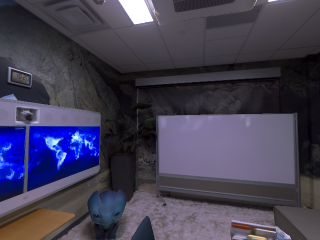
\includegraphics[width=\tw cm,height=\th cm]{keyframe_rgb.png}};
\draw[frm] (rgb.south west) rectangle (rgb.north east);
\node[txt] at (\xA+\wA/2+0.08, \yA-0.33-\th) {posed RGB (+ depth)};

\draw[arr] (\xA+0.55, \yA-0.62-\th) -- (\xA+0.55, \yB+0.06) node[midway, right, lbl] {LSeg};
\node[ttl] at (\xA-0.04, \yB+0.08) {\step{2} features $\zv_p$};
\node[img] (pca) at (\xA, \yB-0.34) {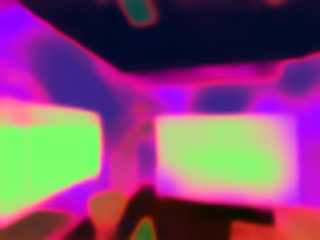
\includegraphics[width=\tw cm,height=\th cm]{features_pca.png}};
\draw[frm] (pca.south west) rectangle (pca.north east);
\node[txt] at (\xA+\wA/2, \yB-0.37-\th)
  {$\zv_p\in\Sph^{d-1}$\\[1pt] PCA $B$,\ $d{=}64$};

% ================================================================== (3) render + backward
\node[evidbox, minimum width=\wB cm, minimum height=\hA cm] (rb) at (\xB, \yA) {};
\node[ttl, text=evidtxt] at (\xB, \yA) {\step{3} one render $+$ backward};
\begin{scope}[shift={(\xB+0.40, \yA-0.70)}, line width=0.35pt]   % 3D-GS glyph (schematic)
  \draw[fill=okblue!35, draw=okblue!70!black, rotate=25]  (0,0) ellipse (0.20 and 0.075);
  \draw[fill=okgreen!35, draw=okgreen!70!black, rotate=-30] (0.27,0.10) ellipse (0.17 and 0.065);
  \draw[fill=okorange!45, draw=okorange!70!black, rotate=60] (0.02,-0.27) ellipse (0.15 and 0.06);
\end{scope}
\node[anchor=west, align=left, inner sep=0.5pt] at (\xB+0.86, \yA-0.70)
  {3D-GS map,\\ geometry fixed};
\node[txt] at (\xB+\wB/2, \yA-1.06)
  {$\Fv_p=\sum_n w_{p,n}\fv_n$\\[2pt]
   $\partial_{\fv_n}\!\sum_p\Yv_p^{\top}\Fv_p$\\[1pt] ${}=\sum_p w_{p,n}\Yv_p$\\[2pt]
   $\Yv_p=[\zv_p,1,\text{depth},\text{mask}]$\\[2pt]
   $\Rightarrow$\ $\R_v$,\ $m_v$,\ depth sums};

% ================================================================== (4) one observation per view
\node[evidbox, minimum width=\wC cm, minimum height=\hA cm] (ob) at (\xC, \yA) {};
\node[ttl, text=evidtxt] at (\xC, \yA) {\step{4} one observation per view};
\begin{scope}[shift={(\xC+\wC/2, \yA-1.12)}]                    % unit-circle glyph (schematic)
  \draw[black!40, line width=0.4pt] (0,0) circle (0.50);
  \foreach \a in {14,30,46,60,74,112} \draw[-{Stealth[length=1.0mm]}, black!45, line width=0.35pt]
    (0,0) -- (\a:0.50);
  \draw[-{Stealth[length=1.6mm]}, evid, line width=1.1pt] (0,0) -- (52:0.38);
  \node[lbl, text=black!60, anchor=west] at (8:0.52) {$\zv_p$};
  \node[lbl, text=evidtxt, anchor=east] at (205:0.10) {$\uv_v$};
\end{scope}
\node[txt] at (\xC+\wC/2, \yA-1.82)
  {$\uv_v=\R_v/m_v$,\ $\lVert\uv_v\rVert\le1$\\[1pt]
   $\omega_v=\min\Big(1,\dfrac{m_v}{a_0HW}\Big)$};

% ================================================================== (5) running sums
\node[evidbox, minimum width=\wD cm, minimum height=\hA cm] (rs) at (\xD, \yA) {};
\node[ttl, text=evidtxt] at (\xD, \yA) {\step{5} running sums};
\node[txt] at (\xD+\wD/2, \yA-0.36)
  {$\R=\sum\omega\uv$\\[1pt]
   $W_1=\sum\omega$\\[1pt] $W_2=\sum\omega^2$\\[1pt]
   $Q=\sum\omega^2\lVert\uv\rVert^2$\\[4pt]
   buckets $\R^{\old}$, $\R^{\new}$:\\[1pt]
   views weighted by $\nu$,\\[1pt] retention $\lambda$};

% ================================================================== (6) posterior + uncertainty
\node[rdbox, minimum width=\wE cm, minimum height=4.30cm] (po) at (\xE, \yA) {};
\node[ttl, text=rdtxt] at (\xE, \yA) {\step{6} posterior, uncertainty};
\node[txt] at (\xE+\wE/2, \yA-0.38)
  {vMF: $\muv^\star=\R/\lVert\R\rVert$\\[1pt] $A_d(\hat\kappa)=\lVert\R\rVert/(W_1{+}c_0)$};
\def\xEa{\xE+0.10} \def\xEb{\xE+\wE-0.10-\sw}
\node[lbl, anchor=south] at (\xEa+\sw/2, \yA-1.32) {epistemic};
\node[lbl, anchor=south] at (\xEb+\sw/2, \yA-1.32) {aleatoric};
\node[img] (ue) at (\xEa, \yA-1.32) {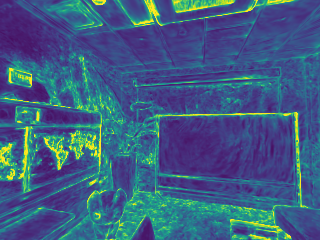
\includegraphics[width=\sw cm,height=\sh cm]{u_epi.png}};
\node[img] (ua) at (\xEb, \yA-1.32) {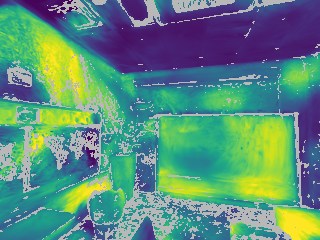
\includegraphics[width=\sw cm,height=\sh cm]{u_ale.png}};
\draw[frm] (ue.south west) rectangle (ue.north east);
\draw[frm] (ua.south west) rectangle (ua.north east);
\node[txt] at (\xE+\wE/2, \yA-1.37-\sh)
  {$u^{\epi}=1/(1{+}s)$,\ $s=W_1$\\[1pt] $u^{\ale}=1-\hat\rho$ if $s\ge\tau_{\min}$};
\node[txt] at (\xE+\wE/2, \yA-3.04)
  {$\hat\rho^{\,2}=\Big[\dfrac{\lVert\R\rVert^2-Q}{W_1^2-W_2}\Big]_0^1$};
% colour key: viridis low..high, grey undefined
\node[lbl, anchor=east, font=\sixpt] at (\xE+0.48, \yA-4.10) {low};
\node[img, anchor=west] (cb) at (\xE+0.50, \yA-4.10)
  {
\includegraphics[width=0.80cm,height=0.12cm]{viridis_strip.png}};
\draw[frm] (cb.south west) rectangle (cb.north east);
\node[lbl, anchor=west, font=\sixpt] at (cb.east) {high};
\fill[undefgrey] (\xE+2.08, \yA-4.16) rectangle ++(0.12, 0.12);
\draw[frm] (\xE+2.08, \yA-4.16) rectangle ++(0.12, 0.12);
\node[lbl, anchor=west, font=\sixpt] at (\xE+2.21, \yA-4.10) {$s<\tau_{\min}$};

% ================================================================== threshold (mapping pass)
\node[chgbox, minimum width=\wB cm, minimum height=\hB cm] (th) at (\xB, \yB) {};
\node[ttl, text=chgtxt] at (\xB, \yB) {threshold $\theta(h)$};
\node[txt] at (\xB+\wB/2, \yB-0.40)
  {null of mapping-pass $\bar c$\\[1pt] per history size $h$};
\node[img, anchor=north] (nh) at (\xB+\wB/2, \yB-1.40)
  {
\includegraphics[width=2.40cm,height=0.76cm]{null_hist.pdf}};
\node[lbl, text=chgtxt, anchor=south, inner sep=0.5pt]
  at ($(nh.north west)!\nullthetafrac!(nh.north east)$) {$\theta(h)$};
\node[txt] at (\xB+\wB/2, \yB-2.24)
  {$\theta(h)$: $q$-quantile, $q{=}0.999$\\[1pt] (nominal $10^{-3}$ per view)};

% ================================================================== (7) change test
\node[chgbox, minimum width=\wC cm, minimum height=\hB cm] (ct) at (\xC, \yB) {};
\node[ttl, text=chgtxt] at (\xC, \yB) {\step{7} change test (each view)};
\node[img] (chi) at ({\xC+(\wC-\tw)/2}, \yB-0.34)
  {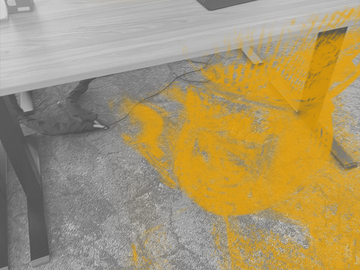
\includegraphics[width=\tw cm,height=\th cm]{change_nor002.png}};
\draw[frm] (chi.south west) rectangle (chi.north east);
\node[img, anchor=north west] (chb) at ($(chi.north west)+(0.04,-0.04)$)
  {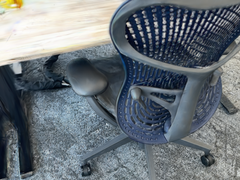
\includegraphics[width=0.86cm,height=0.645cm]{change_nor002_before.png}};
\draw[white, line width=0.6pt] (chb.south west) rectangle (chb.north east);
\node[font=\sixpt, anchor=north west, inner sep=0.6pt, fill=white, fill opacity=0.85,
  text opacity=1] at (chb.south west) {before};
\node[font=\sixpt, anchor=south east, inner sep=0.6pt, fill=white, fill opacity=0.85,
  text opacity=1] at (chi.south east) {after: reset};
\node[txt] at (\xC+\wC/2, \yB-1.97)
  {$c=1-\cos(\R^{\old},\R^{\new})$\\[1.5pt]
   $\bar c$: min of last $k$;\ $\lambda{=}0$, $k{=}2$\\[1.5pt]
   fires if $\bar c>\theta(h)$};

% ================================================================== (8) reset, re-admission
\node[chgbox, minimum width=\wD cm, minimum height=\hB cm] (rr) at (\xD, \yB) {};
\node[ttl, text=chgtxt] at (\xD, \yB) {\step{8} reset, re-admission};
\node[txt] at (\xD+\wD/2, \yB-0.42)
  {fired: the sums restart\\[1pt] from this view; \emph{changed}\\[5pt]
   re-admit once $\nu\ge3$ since\\[1pt] the reset and the mean\\[1pt]
   $\lvert d^{\mathrm{obs}}{-}d^{\mathrm{ctr}}\rvert\le5$\,cm\\[1pt]
   {\sixpt(observed vs.\ centre depth)}};

% ================================================================== robust set
\node[rdbox, minimum width=\wE cm, minimum height=1.12cm] (rob) at (\xE, \yB-1.45) {};
\node[ttl, text=rdtxt] at (\xE, \yB-1.45) {robust set};
\node[txt] at (\xE+\wE/2, \yB-1.83)
  {$s\ge\tau_{\min}$,\ \ $\hat\rho\ge0.6$,\\[1pt] not \emph{changed}};

% ================================================================== (9) predictive render
\node[rdbox, minimum width=\wF cm, minimum height=6.20cm] (pr) at (\xF, \yA) {};
\node[ttl, text=rdtxt] at (\xF, \yA) {\step{9} predictive};
\node[txt] at (\xF+\wF/2, \yA-0.38)
  {$\tv_c=B^{\top}\tilde\tv_c$\\[2pt]
   $P(y_p{=}c)=$\\[0.5pt] $\operatorname{softmax}_c(\beta\,\Fv_p^{\top}\tv_c)$\\[3pt]
   P0: $\fv_n=\muv^\star_n$\\[1pt]
   P1: $\fv_n=\mathbb{E}[\muv_n]$\\[1pt]
   P2: P0 with\\[1pt] $\beta_p(u^{\epi}_p,u^{\ale}_p)$};
\node[img] (lab) at ({\xF+(\wF-\tw)/2}, \yA-3.02)
  {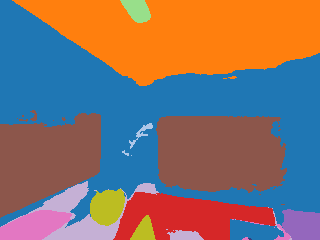
\includegraphics[width=\tw cm,height=\th cm]{labels_p2.png}};
\draw[frm] (lab.south west) rectangle (lab.north east);
\node[txt] at (\xF+\wF/2, \yA-3.05-\th) {P2 labels (argmax)};
\begin{scope}[shift={(\xF+0.16, \yA-5.15)}]
  \foreach \c/\n/\dx/\dy in {labA/\labnameA/0/0, labB/\labnameB/1.10/0,
                             labC/\labnameC/0/-0.27, labD/\labnameD/1.10/-0.27} {
    \fill[\c] (\dx, \dy-0.06) rectangle ++(0.12, 0.12);
    \draw[frm] (\dx, \dy-0.06) rectangle ++(0.12, 0.12);
    \node[lbl, anchor=west, font=\sixpt, inner sep=0.5pt] at (\dx+0.14, \dy) {\n};
  }
\end{scope}
\draw[arr] (\xF+\wF/2, \yA+0.42) node[above, lbl, inner sep=0.5pt] {text query $\tilde\tv_c$}
  -- (\xF+\wF/2, \yA+0.02);

% ================================================================== arrows
\def\ym{-1.15}
\draw[arr] (rgb.east |- 0,\ym) -- (\xB, \ym);
\draw[arr] (pca.east) -- ++(0.20,0) |- (\xB, -2.40);
\draw[arr] (\xB+\wB, \ym) -- (\xC, \ym);
\draw[arr] (\xC+\wC, \ym) -- (\xD, \ym);
\draw[arr] (\xD+\wD, \ym) -- (\xE, \ym);
\draw[arr] (\xE+\wE, \ym) -- (\xF, \ym);
% the current view against all earlier evidence
\draw[chgarr] (\xC+0.55, \yA-\hA) -- (\xC+0.55, \yB) node[midway, right, lbl, text=chgtxt] {$\nu_v\uv_v$};
\draw[chgarr, rounded corners=2pt] (\xD+0.45, \yA-\hA) -- (\xD+0.45, \yA-\hA-0.21)
  -- (\xC+\wC-0.45, \yA-\hA-0.21) -- (\xC+\wC-0.45, \yB);
\node[lbl, text=chgtxt, anchor=south, inner sep=0.5pt] at (\xC+\wC-0.05, \yA-\hA-0.21) {$\R^{\old}$};
% threshold: mapping-pass scores in, theta(h) out (update pass)
\draw[arr, black!55, line width=0.45pt] (\xC, \yB-1.05) -- (\xB+\wB, \yB-1.05);
\draw[chgarr] (\xB+\wB, \yB-1.62) -- (\xC, \yB-1.62);
% fire -> reset; reset -> sums; flag -> robust set; s, rho -> robust set
\draw[chgarr] (\xC+\wC, \yB-1.20) -- (\xD, \yB-1.20);
\draw[chgarr, line width=0.9pt] (\xD+1.95, \yB) -- (\xD+1.95, \yA-\hA)
  node[midway, right, lbl, text=chgtxt] {reset};
\draw[chgarr] (\xD+\wD, \yB-2.00) -- (\xE, \yB-2.00);
\draw[arr, draw=rd] (\xE+\wE/2, \yA-4.30) -- (\xE+\wE/2, \yB-1.45)
  node[midway, right, lbl, text=rdtxt] {$s$, $\hat\rho$};
\end{tikzpicture}
\end{document}
